\documentclass[
	article,
	12pt,
	oneside,
	a4paper,
	english,
	brazil,
	sumario=tradicional
]{abntex2}

% Pacotes fundamentais
\usepackage{times}
\usepackage[T1]{fontenc}
\usepackage[utf8]{inputenc}
\usepackage{indentfirst}
\usepackage{color}
\usepackage{graphicx}
\usepackage{amsmath}
\usepackage{gensymb}
\usepackage{lscape}
\usepackage{pdflscape}
\usepackage[table,xcdraw]{xcolor}
\usepackage{float}
\usepackage{microtype}
\usepackage{multirow}
\usepackage[normalem]{ulem}
\usepackage{rotating}
\usepackage{booktabs}
\usepackage[alf,abnt-etal-cite=3,abnt-etal-list=0]{abntex2cite}
\usepackage{hyperref}
\usepackage{tabularx} % For tabularx environment
\usepackage{booktabs} % For \toprule, \midrule, and \bottomrule
\usepackage{caption} % For \captionsetup
\usepackage{makecell}
\newcommand{\theforeigntitle}[1]{\def\@theforeigntitle{#1}}

% Configurações de aparência do PDF final
\definecolor{blue}{RGB}{41,5,195}
\hypersetup{
	pdftitle={Trabalho final de Econometria III - Replicação do artigo "Political systems, regime memory, and economic freedom"},
	pdfauthor={Bruno Francisco Schaden},
	pdfsubject={Modelo de artigo científico com abnTeX2},
	pdfcreator={LaTeX with abnTeX2},
	pdfkeywords={abnt}{latex}{abntex}{abntex2}{artigo científico},
	colorlinks=true,
	linkcolor=blue,
	citecolor=blue,
	filecolor=magenta,
	urlcolor=blue,
	bookmarksdepth=4
}

% Configurações de margens
\setlrmarginsandblock{3cm}{2cm}{*}
\setulmarginsandblock{3cm}{2cm}{*}
\checkandfixthelayout

% Espaçamentos entre linhas e parágrafos
\setlength{\parindent}{1.5cm}
\setlength{\parskip}{0.2cm}
\OnehalfSpacing

% Informações de dados para CAPA e FOLHA DE ROSTO
\titulo{Trabalho final de Econometria III - Replicação do artigo "Political systems, regime memory, and economic freedom"}
\autor{Bruno Francisco Schaden}
\local{Florianópolis}
\data{2024}

\begin{document}

\frenchspacing

% ELEMENTOS PRÉ-TEXTUAIS
\maketitle
\selectlanguage{english}

% Resumo em inglês
	\begin{resumoumacoluna}
	\noindent
	The article "Political systems, regime memory and economic freedom" by Peter Calcagno, Beatriz Maldonado, Todd Nesbit and Mary Frances Zeager investigates the influence of the memory of past regimes on a country's economic freedom. The authors develop an innovative measure of regime memory and analyze the generational effect of previous regimes on economic freedom. Through a study of 144 countries between 1970 and 2015, the article highlights that regime memory can promote improvements in economic freedom in historically democratic nations, while discouraging it in countries with an autocratic history. These results contribute to the understanding of how past culture, traditions and institutions impact current economic policies.
	
	\textbf{Keywords:} Political systems. Regime memory. Economic freedom. Culture. Institutions.
	
	\textbf{JEL Classification: P16, P48, N40, O43}
	\end{resumoumacoluna}

\newpage

\selectlanguage{brazil}
% Resumo em português
\renewcommand{\resumoname}{Resumo}
\begin{resumoumacoluna}
\begin{otherlanguage*}{brazil}
   \noindent 
   O artigo "Sistemas políticos, memória de regime e liberdade econômica" de Peter Calcagno, Beatriz Maldonado, Todd Nesbit e Mary Frances Zeager investiga a influência da memória de regimes passados na liberdade econômica de um país. Os autores desenvolvem uma medida inovadora de memória de regime e analisam o efeito geracional de regimes anteriores na liberdade econômica. Por meio de um estudo com 144 países entre 1970 e 2015, o artigo destaca que a memória de regime pode promover melhorias na liberdade econômica em nações historicamente democráticas, enquanto desencoraja em países com histórico autocrático. Esses resultados contribuem para a compreensão de como a cultura, as tradições e as instituições passadas impactam as políticas econômicas atuais.   
   
   \textbf{Palavras-chave}: Sistemas políticos. Memória de regime. Liberdade Econômica. Cultura. Instituições.
   
   \textbf{Classificação JEL: P16, P48, N40, O43}
 \end{otherlanguage*}  
\end{resumoumacoluna}

\newpage


% ELEMENTOS TEXTUAIS
\textual


%\chapter{Introdução}


\chapter{Do Artigo Científico de Replicação}

O estudo de Calcagno et al. (2024) explora como sistemas políticos e a memória de regimes anteriores influenciam a liberdade econômica atual. A liberdade econômica é um conceito crítico que afeta o desenvolvimento econômico e social dos países. Este trabalho objetiva replicar os métodos e resultados de Calcagno et al. (2024) para confirmar a robustez das suas conclusões.

A motivação para esta replicação reside na importância de verificar a reprodutibilidade das pesquisas acadêmicas. Estudos replicados com sucesso reforçam a validade das teorias propostas e aumentam a confiança na literatura científica existente. A abordagem metodológica e os dados utilizados são detalhados nas seções subsequentes.


\section{Fonte dos Dados}
Os dados utilizados nesta replicação são provenientes das mesmas fontes mencionadas por Calcagno et al. (2024). Utilizamos o dataset replicação composto de liberdade econômica do Fraser Institute (2022) e variáveis políticas do Polity IV Project. Estes conjuntos de dados fornecem uma cobertura ampla e detalhada de indicadores econômicos e políticos ao longo do tempo.

Adicionalmente, também é incorporado no dataset dados demográficos e econômicos do Banco Mundial para controlar variáveis que possam influenciar a liberdade econômica. Estes dados permitem uma análise comparativa robusta entre diferentes países e regimes ao longo das últimas décadas.

\section{Memória de Regime}
A metodologia replicada segue os passos descritos por Calcagno et al. (2024) somente mudando o softwere de análise de Stata para Python. Utilizamos modelos de regressão linear múltipla para analisar a relação entre sistemas políticos, memória de regime e liberdade econômica. A variável dependente é o índice de liberdade econômica, enquanto as variáveis independentes incluem indicadores políticos e demográficos.

Para capturar os efeitos das mudanças institucionais lentas associadas à mudança de regime, utilizamos duas variáveis para construir nossa medida de memória de regime. Durable é uma variável de contagem que registra o tempo desde a mudança de regime mais recente. Para registrar um efeito na memória de regime, a pontuação máxima de durable para um determinado regime deve ser maior que zero. Polity2 controla o tipo de regime e varia de -10 a 10, com uma pontuação mais baixa indicando um regime mais autocrático e uma pontuação maior indicando um regime mais democrático.

Nossa medida de memória de regime de um país é melhor descrita como uma média ponderada das pontuações de polity2 pelo regime em que os pesos são determinados pela pontuação de durable de cada regime. A construção ampla é descrita da seguinte forma:

\[
\text{RegimeMemory}_{it} = \frac{\sum_{r=0}^{R} \left( w_{(t-1)r} \cdot \text{Polity2}_{(t-1-k)r} \right)}{\sum_{r=0}^{R} w_{(t-1)r}}
\]

onde $i$ e $t$ são índices para país e ano, respectivamente, e $r$ é o índice para o regime. Todas as referências temporais no lado direito são defasadas de modo que a memória de regime não é influenciada diretamente pelas pontuações contemporâneas de polity e durable — ela é destinada a representar puramente a memória dos regimes passados. O subscrito $k$ indexa o número de anos desde o término do regime anterior. Os pesos dos regimes são atribuídos com um valor inicial de um no primeiro ano de existência do regime. A influência desse regime, e portanto seu peso, é assumida como crescente a uma taxa de desconto constante (2,5\% e 12,5\% para os resultados principais apresentados aqui) a cada ano adicional em que o regime está em vigor. Uma vez que um regime termina, o peso atribuído à contribuição desse regime para a memória de regime começa a diminuir na mesma taxa de desconto. Nosso período de amostra para nossa análise de regressão começa em 1970; no entanto, a medida de memória de regime para um determinado país inclui a influência descontada de todos os regimes passados incluídos no conjunto de dados Polity IV.

\begin{figure}[h!]
    \centering
    \caption{Variável de memória de regime para Chile e França entre 1970 e 2015, utilizando taxas de desconto de 2,5\% e 12,5\%, assim como a medida de cálculo alternativa.}
    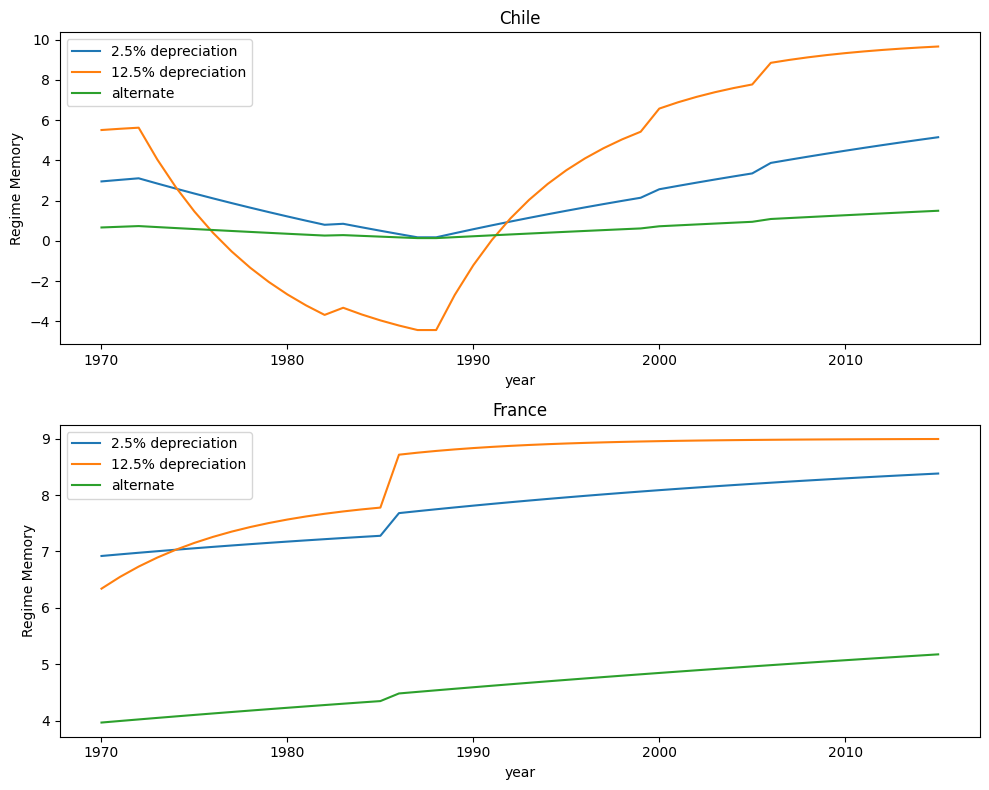
\includegraphics[width=0.8\textwidth]{Textuais/chile.png}
    \fonte{Replicação - Elaborado pelos autores.}
\end{figure}

\section{Metodologia Empírica}

A análise de regressão realizada utiliza o modelo de efeitos fixos para examinar a relação entre memória de regime e liberdade econômica. Este modelo permite controlar variáveis não observadas que são constantes ao longo do tempo, mas variam entre os países. A especificação do modelo é dada pela seguinte equação:

\begin{equation}
    \text{EFW}_{it} = \beta_1 \text{RegimeMemory}_{it} + \mathbf{X}_{it-1} \boldsymbol{\delta} + \Phi_t + \epsilon_{it} \quad 
\end{equation}

onde $i$ representa o índice de país e $t$ representa o índice de ano. Para explicar como a memória de regime afeta a liberdade econômica de um país, utilizamos o índice de Liberdade Econômica do Mundo (EFW) do projeto Economic Freedom of the World como nossa medida de liberdade econômica (Gwartney et al., 2022). O índice varia de 0 a 10, com pontuações mais baixas denotando menos liberdade econômica e pontuações mais altas denotando mais liberdade.


\chapter{Resultados}

\section{Descrição dos Dados}
As estatísticas descritivas das variáveis foram reproduzidas quase perfeitamente, como mostrado na Tabela \ref{tab:tabela_descritiva}. A diferença encontrada nos números é de orderm de $10^{-2}$, o que é aceitável dada a natureza dos cálculos. 

\begin{table}[htbp]
    \centering
    \renewcommand{\arraystretch}{1.1}
    \captionsetup{font=small}
    \caption{Estatísticas Descritivas.}
    \label{tab:tabela_descritiva}
    \scriptsize % Ajusta a fonte para tamanho 10
    \begin{tabular}{lrrrrrrrr}
        \toprule
        \textbf{Variável} & \textbf{N} & \textbf{Média} & \textbf{Desv. Padrão} & \textbf{Mín.} & \textbf{25\%} & \textbf{50\%} & \textbf{75\%} & \textbf{Máx.} \\
        \midrule
        EFW index interpolated & 4697 & 6.14 & 1.30 & 2.37 & 5.18 & 6.20 & 7.18 & 8.85 \\
        EFW index not interpolated & 2534 & 6.53 & 1.16 & 2.37 & 5.75 & 6.65 & 7.44 & 8.85 \\
        2.5\% discount & 4697 & 0.38 & 6.05 & -10.0 & -4.93 & -0.54 & 6.00 & 10.0 \\
        5\% discount & 4697 & 1.01 & 6.34 & -10.0 & -4.84 & 0.79 & 7.00 & 10.0 \\
        7.5\% discount & 4697 & 1.43 & 6.51 & -10.0 & -4.72 & 2.01 & 7.90 & 10.0 \\
        10\% discount & 4697 & 1.73 & 6.64 & -10.0 & -4.65 & 3.03 & 8.03 & 10.0 \\
        12.5\% discount & 4697 & 1.95 & 6.73 & -10.0 & -4.59 & 3.70 & 8.61 & 10.0 \\
        15\% discount & 4697 & 2.10 & 6.79 & -10.0 & -4.63 & 4.00 & 8.89 & 10.0 \\
        Alternative & 4697 & 0.27 & 6.20 & -10.0 & -4.93 & 0.69 & 4.30 & 10.0 \\
        Net ODA as \% of GDP & 4697 & 3.28 & 5.59 & -0.40 & 0.00 & 0.69 & 3.07 & 81.43 \\
        Resource rent as \% of GDP & 4697 & 7.05 & 9.75 & 0.00 & 0.00 & 3.07 & 9.21 & 79.74 \\
        Real GDP per capita & 4697 & 11224.56 & 16503.12 & 157.10 & 1262.87 & 3731.68 & 14263.96 & 114047.91 \\
        GDP growth & 4697 & 3.67 & 4.94 & -50.25 & -4.93 & 0.79 & 7.00 & 39.49 \\
        War Dummy & 4697 & 0.09 & 0.28 & 0 & 0 & 0 & 0 & 1 \\
        Christian Dummy & 4697 & 0.63 & 0.48 & 0 & 0 & 1 & 1 & 1 \\
        UK legal origin & 4697 & 0.30 & 0.46 & 0 & 0 & 0 & 1 & 1 \\
        French legal origin & 4697 & 0.56 & 0.50 & 0 & 0 & 1 & 1 & 1 \\
        Coup d'etats & 4477 & 0.04 & 0.21 & 0 & 0 & 0 & 0 & 1 \\
        Gini & 3530 & 39.07 & 8.84 & 20.30 & 32.40 & 39.60 & 45.07 & 65.40 \\
        \bottomrule
    \end{tabular}
    \fonte{Elaborado pelos autores.}
\end{table}


\section{SEÇÃO SECUNDÁRIA}

A ABNT indica a elaboração de uma lista de ilustrações com todos os itens arrolados e designados por seu nome específico, conforme a ordem que aparecem no texto (Figura 1, Fotografia 1, Gráfico 1, Quadro 1, entre outros). Também recomenda, quando necessário, a elaboração de lista própria para cada tipo de ilustração. No entanto, não determina um número mínimo de ilustrações para tal lista específica.

\begin{table}
	\caption{Tabela 3 do Artigo Original.}
	\label{tab:tabela3}
	\resizebox{\textwidth}{!}{\begin{tabular}{lcccc}
	\toprule
	Dependent variable & EFW index-interpolate (2.50\%) & EFW index-interpolate (12.50\%) & EFW index (2.50\%) & EFW index (12.50\%) \\
	\midrule
	Regime memory & 0.043 & 0.045 & 0.024 & 0.037 \\
	Net ODA as \% of GDP & 0.020 & 0.020 & 0.021 & 0.021 \\
	Resource rent as \% of GDP & -0.023 & -0.021 & -0.028 & -0.024 \\
	ln(GDP per capita) & 0.492 & 0.499 & 0.476 & 0.468 \\
	GDP Growth & 0.019 & 0.019 & 0.021 & 0.020 \\
	War Dummy & -0.234 & -0.209 & -0.195 & -0.200 \\
	Christian Dummy & -0.143 & -0.185 & 0.029 & -0.051 \\
	British legal origin & 0.089 & 0.162 & 0.125 & 0.177 \\
	French legal origin & -0.065 & -0.047 & -0.040 & -0.019 \\
	Number of observations & 4697 & 4697 & 2534 & 2534 \\
	R2 & 0.732 & 0.738 & 0.730 & 0.742 \\
	\bottomrule
	\end{tabular}}
	\end{table}


	\begin{table}
		\caption{Tabela 4 do Artigo Original.}
		\label{tab:tabela4}
		\resizebox{\textwidth}{!}{\begin{tabular}{lcccc}
		\toprule
		Dependent variable & EFW index-interpolate (2.50\%) & EFW index-interpolate (12.50\%) & EFW index (2.50\%) & EFW index (12.50\%) \\
		\midrule
		Regime memory & 0.045 & 0.046 & 0.045 & 0.050 \\
		Net ODA as \% of GDP & 0.021 & 0.021 & 0.021 & 0.022 \\
		Resource rent as \% of GDP & -0.023 & -0.021 & -0.026 & -0.023 \\
		ln(GDP per capita) & 0.485 & 0.493 & 0.464 & 0.481 \\
		GDP Growth & 0.020 & 0.019 & 0.032 & 0.032 \\
		War Dummy & -0.244 & -0.222 & -0.193 & -0.167 \\
		Christian Dummy & -0.132 & -0.178 & -0.049 & -0.113 \\
		British legal origin & 0.077 & 0.156 & 0.061 & 0.148 \\
		French legal origin & -0.072 & -0.050 & -0.143 & -0.120 \\
		Coup Dummy & -0.039 & -0.021 & -0.131 & -0.102 \\
		Gini Disposable & NA & NA & 0.002 & 0.004 \\
		Number of observations & 4477 & 4477 & 3462 & 3462 \\
		R2 & 0.727 & 0.733 & 0.714 & 0.724 \\
		\bottomrule
		\end{tabular}}
		\end{table}
Nesse caso, a BU Udesc estabelece a elaboração de listas específicas para cada tipo de ilustração somente quando existirem muitos itens de cada tipo: cinco (5) ou mais (mais do que cinco desenhos, gráficos etc.). Caso contrário, elabora-se uma única lista, denominada “Lista de ilustrações” com os elementos ordenados conforme aparecem no texto, nominando-os “Figura” e, portanto, não diferenciando fotografia, gráfico, quadro e outros.


\subsection{Seção terciária}

O vídeo fornece uma maneira poderosa de ajudá-lo a provar seu argumento. Ao clicar em Vídeo Online, você pode colar o código de inserção do vídeo que deseja adicionar.

\subsubsection{Seção quaternária}

O vídeo fornece uma maneira poderosa de ajudá-lo a provar seu argumento. Ao clicar em Vídeo Online, você pode colar o código de inserção do vídeo que deseja adicionar. Você também pode digitar uma palavra-chave para pesquisar online o vídeo mais adequado ao seu documento. 


\begin{figure}
	\centering
	\caption{Exemplo de paginação.}
	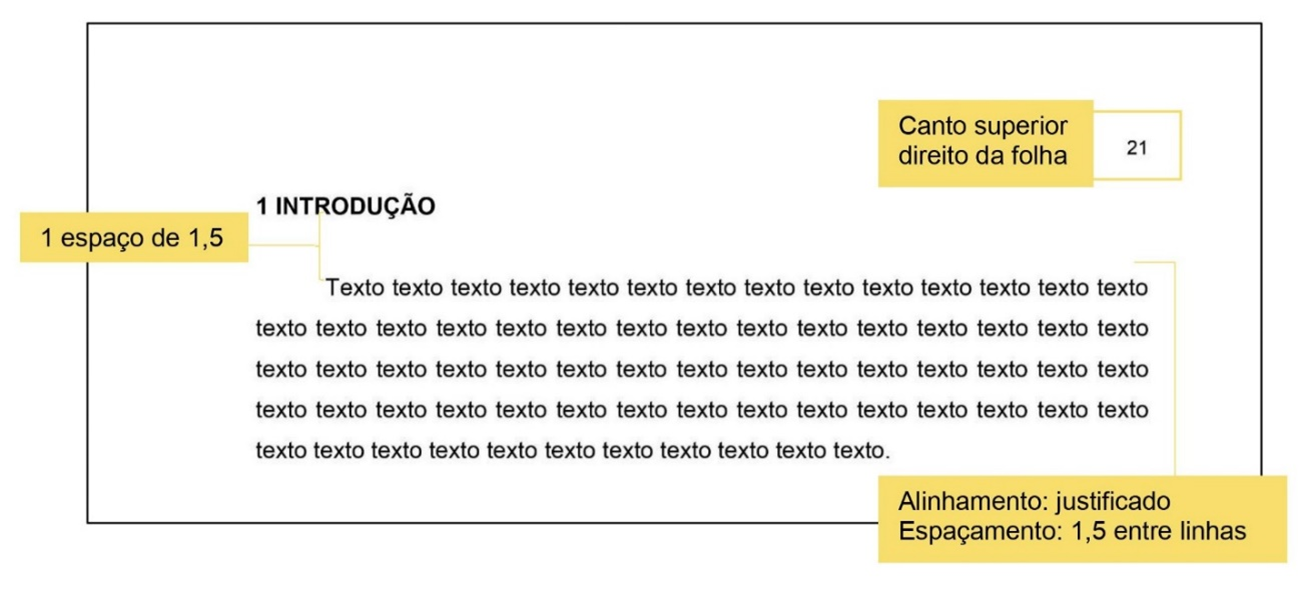
\includegraphics[scale=1]{Textuais/Picture1.png}
	\fonte{Elaborada pelos autores (2020), com base na NBR 14724 (2011).}
\end{figure}


\subsubsubsection{Seção quinaria}



O vídeo fornece uma maneira poderosa de ajudá-lo a provar seu argumento. Ao clicar em Vídeo Online, você pode colar o código de inserção do vídeo que deseja adicionar. Você também pode digitar uma palavra-chave para pesquisar online o vídeo mais adequado ao seu documento. Para dar ao documento uma aparência profissional, o Word\footnote{O Microsoft Word é um processador de texto produzido pela Microsoft Office foi criado por Richard Brodie para computadores IBM PC com o sistema operacional DOS em 1983.} fornece designs de cabeçalho, rodapé, folha de rosto e caixa de texto que se complementam entre si. Por exemplo, você pode adicionar uma folha de rosto, um cabeçalho e uma barra lateral correspondentes.

\begin{table}[!htbp]
	\centering
	%	\small
	\renewcommand{\arraystretch}{1.1}
	\caption{Modelo de tabela.}%
	\label{tab:tabela_exemplo}
	\begin{tabular}{ L{4cm}  R{3cm} || L{4cm}  R{3cm}  }
		\hline
		Município		& População Estimada & Município		& População Estimada 		\\ 
		\hline
		Abdon Batista		& 2630	& Bom Jesus				& 2821 \\ 
		Abelardo Luz		& 17717	& Bom Jesus do Oeste	& 2156 \\ 
		Agrolândia			& 10272	& Bom Retiro			& 9598 \\ 
		Agronômica			& 5306	& Bombinhas				& 17477 \\ 
		Água Doce			& 7132	& Botuverá				& 4943 \\ 
		Águas de Chapecó	& 6379	& Braço do Norte		& 31765 \\ 
		\hline
	\end{tabular}
	\vspace{2mm}
	\fonte{Adaptado de IBGE (2015).}
\end{table}

Clique em Inserir e escolha os elementos desejados nas diferentes galerias.

\begin{figure}
	\centering
	\caption{População.}
	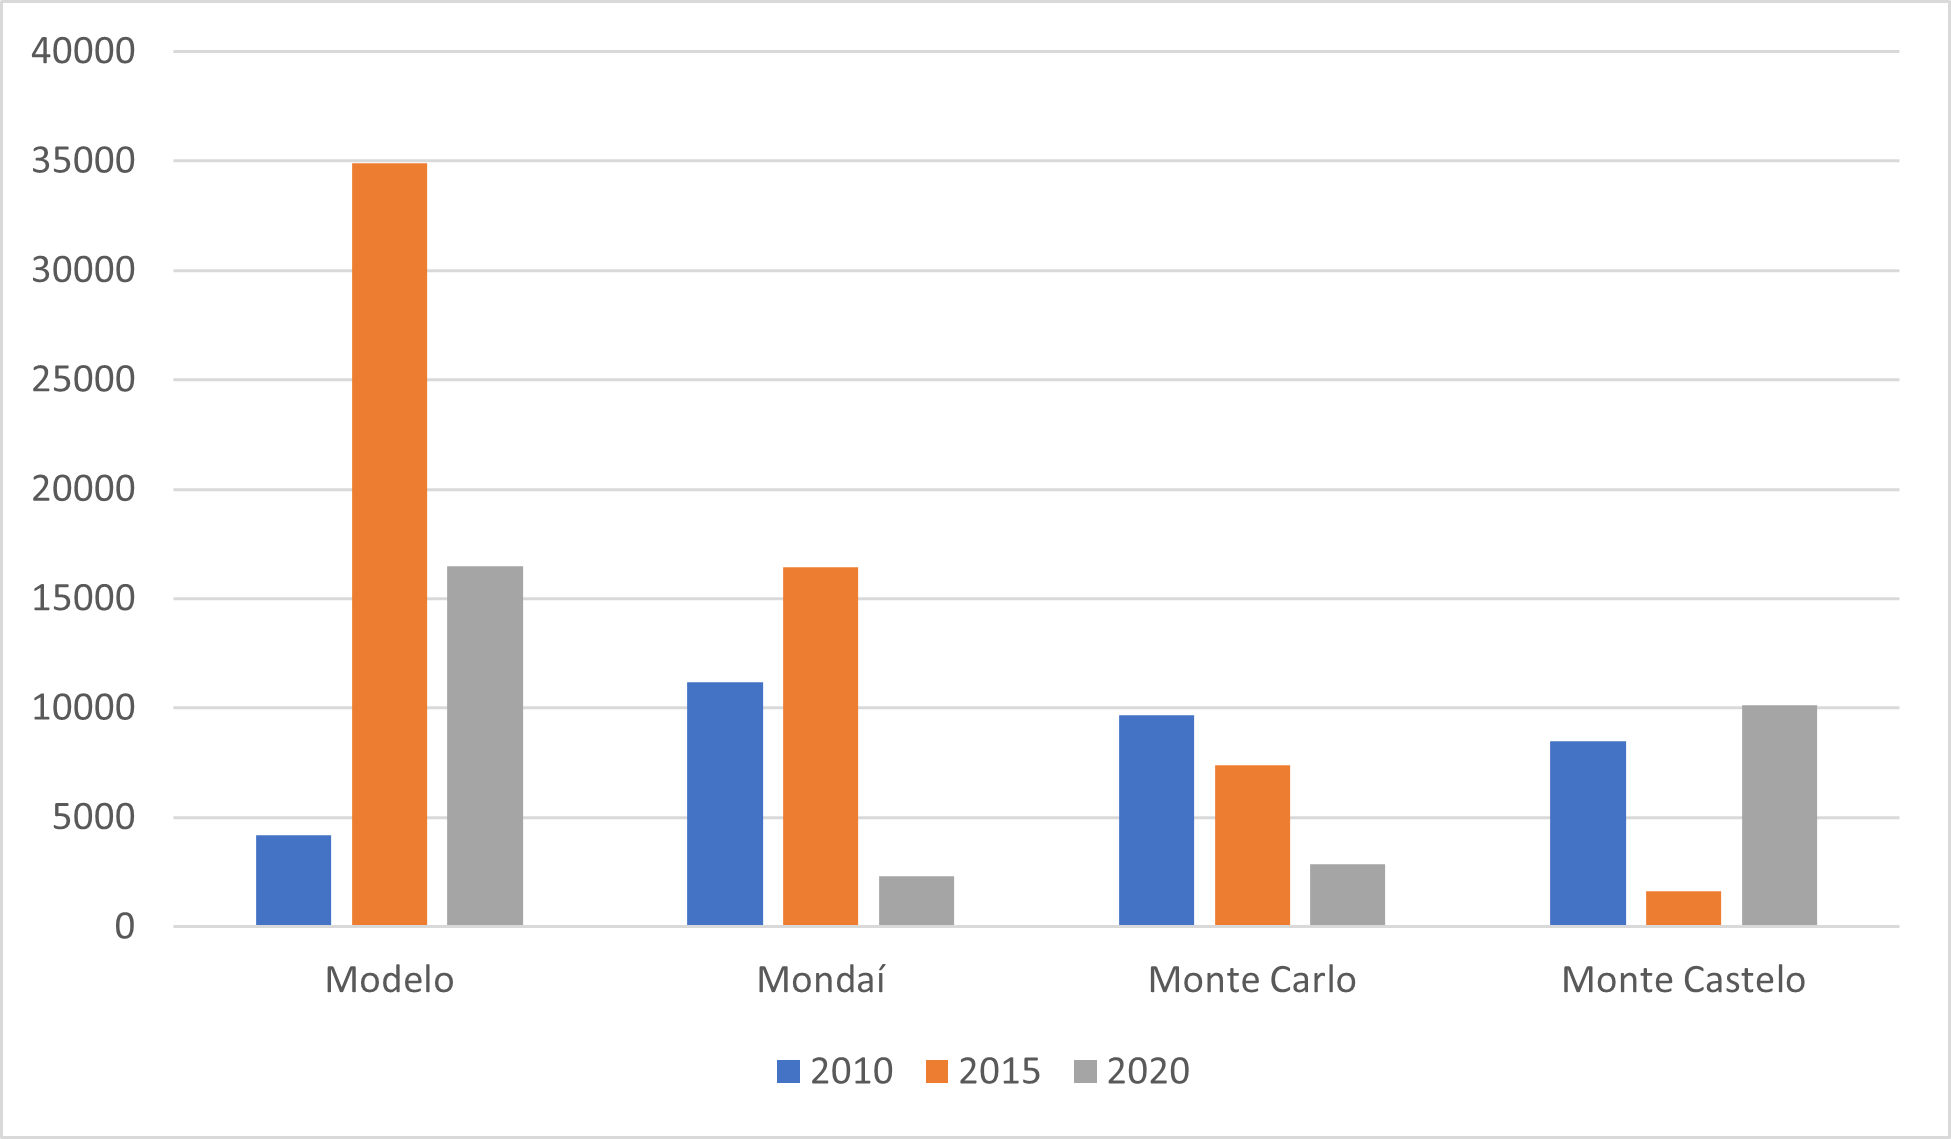
\includegraphics[scale=1]{Textuais/Picture2.png}
	\fonte{\me{2020}}
\end{figure}

As chamadas às equações e fórmulas, no texto, devem ser feitas da seguinte forma: equação (1), fórmula (2).

\textbf{Exemplo 1:}
O Teorema de Pitágoras, é uma equação \eqref{eq:eq1} que pode ser aplicada em qualquer triângulo retângulo (triângulo que tem um ângulo de 90°).
\begin{equation} \label{eq:eq1}
a^2 + b^2 = c^2 
\end{equation}

\textbf{Exemplo 2:}
A dopamina é um composto orgânico de função mista álcool, fenol e amina que apresenta fórmula \eqref{eq:form1} molecular:
\begin{equation} \label{eq:form1}
\ch{C8 + H11NO2} 
\end{equation}

\textbf{Exemplo 3:}
O modelo matemático de Huang (HUG), dado pelas equações \eqref{eq:eq3} e \eqref{eq:eq4}, foi elaborado com o intuito de fornecer uma descrição mais simples do crescimento bacteriano.
\begin{gather} 
	y(t) = y_0 + y_{max} -\ln{[e^{y_0}  + (e^{y_{max}} -e^{y_0} )  e^{-u_{max}\beta(t)} ]}   \label{eq:eq3}  \\
	\beta(t) = t + \frac{1}{4}\ln\left( \frac{1+ e^{-4(t-\lambda)} }{1+ e^{4(\lambda)} }\right) \label{eq:eq4}
\end{gather}
\noindent onde $y(t)$ corresponde ao logaritmo natural da concentração celular (log UFC/g) no instante $t$ (dias), $y_{max}$ é o logaritmo natural da população bacteriana (log UFC/g) final, $y_0$ corresponde ao logaritmo natural da população bacteriana inicial (log UFC/g) e $\beta(t)$ é a função de transição.

\textbf{Exemplo 4:}
Para o cálculo da intensidade fórmula \eqref{eq:eq5} de Intensidade-Duração-Frequência apresentada, os valores encontrados seguindo os parâmetros apresentados e como o resultado é dado em mm/h haverá também a sua conversão para m/s.
\begin{gather} 
	i = \frac{K T^m}{(t+b)^n}   \label{eq:eq5}  \\[2ex]
		i = \frac{\num{625.58} \cdot 5^{\num{0.171}}  }{(60+\num{8.89})^{\num{0.961}}} \\[2ex]
		i = \num{44.222} \cdot \frac{\si{mm}}{\si{h}} \cdot \frac{1\mathrm{m}}{\SI{1000}{mm}} \cdot \frac{\SI{1}{h}}{\SI{3600}{s}} 	
\end{gather}
\noindent onde, $i$ é a intensidade média máxima de precipitação, em mm/h; $T$ é o Período de retorno, em anos; $t$ é a duração da chuva, em minutos; $k,m,b,n$ são os parâmetros da equação determinados para cada local.


As citações diretas com até três linhas ``[...] devem estar contidas entre aspas duplas. As aspas simples são utilizadas para indicar citação no interior da citação.'' (ABNT, 2002, p. 2). Devem apresentar autor, ano e página. Quando a indicação de autor estiver dentro de parênteses, o sobrenome deve ser em letra maiúscula. 


As citações diretas com mais três linhas ``[...] devem ser destacadas com recuo de 4 cm da margem esquerda, com letra menor que a do texto utilizado e sem as aspas.'' (ABNT, 2002, p. 2). Ou seja, utilizar fonte tamanho 10 para as citações diretas longas, com espaçamentos simples entre linhas. As citações devem ser precedidas e antecedidas por um (1) espaço de 1,5 entrelinhas. 

\begin{citacao}
Texto texto texto texto texto texto texto texto texto texto texto texto texto texto texto texto texto texto texto texto texto texto texto texto texto texto texto texto texto texto texto texto texto texto texto texto texto texto texto texto texto texto texto texto texto texto. (SILVA, 2020, p. 21).
\end{citacao}


Nas citações indiretas não há necessidade de usar aspas e indicar a página, considerando que é uma paráfrase. Faz-se necessário apresentar o autor e ano.






\noindent Exemplo referência de livro: \cite{exemplo_livro}

\noindent Exemplo referência de livro em meio eletrônico: \cite{exemplo_livroe}

\noindent Exemplo referência de trabalho acadêmico (Dissertação de Mestrado): \cite{exemplo_dissertacao}

\noindent Exemplo referência de trabalho acadêmico (Tese de Doutorado): \cite{exemplo_tese}

\noindent Exemplo referência de artigo: \cite{exemplo_artigo}


\textbf{Para outras referências ver Manual Udesc}: \url{https://www.udesc.br/bu/manuais}










% ELEMENTOS PÓS-TEXTUAIS
\renewcommand{\refname}{Referências}
\bibliographystyle{abntex2-alf}
\bibliography{abntex2-ref_UDESC_2020}

\end{document}
